\documentclass[a4paper,11pt]{article}

\usepackage[utf8]{inputenc}
\usepackage[swedish]{babel}
\usepackage[top=1in,bottom=1in,left=1in,right=1in,headsep=.5in]{geometry}
\usepackage{hyperref}
\usepackage{graphicx}

\usepackage{array}
\newcolumntype{L}[1]{>{\raggedright\let\newline\\\arraybackslash\hspace{0pt}}m{#1}}
\newcolumntype{C}[1]{>{\centering\let\newline\\\arraybackslash\hspace{0pt}}m{#1}}
\newcolumntype{R}[1]{>{\raggedleft\let\newline\\\arraybackslash\hspace{0pt}}m{#1}}

\usepackage[yyyymmdd,hhmmss]{datetime}
\renewcommand{\dateseparator}{-}

\usepackage{mathptmx}    %Times Roman font
\usepackage{helvet}    %Helvetica, served as a model for arial
\usepackage{anyfontsize}

\usepackage[tocgraduated]{tocstyle}
\usetocstyle{allwithdot}

\usepackage[titletoc,title]{appendix}

\usepackage[backend=bibtex,style=authoryear,maxcitenames=2,maxbibnames=9]{biblatex} %Harvard-style citations
\setlength{\bibitemsep}{\baselineskip}	%vertical space between bibliography items

\usepackage{fancyhdr}
\fancypagestyle{intro}{
    \fancyhf{}
    \fancyhead[C]{\LIPSprojekttitel}
    \fancyhead[R]{\today} 
    \fancyfoot[L]{\LIPSkursnamn \\ \LIPSdokumenttyp}
    \fancyfoot[C]{\phantom{text}\roman{page}}
    \fancyfoot[R]{\LIPSprojektgrupp \\ \LIPSgruppepost} 
    \renewcommand{\headrulewidth}{0.4pt}
    \renewcommand{\footrulewidth}{0.4pt}}
\fancypagestyle{content}{
    \fancyhf{}
    \fancyhead[C]{\LIPSprojekttitel}
    \fancyhead[R]{\today} 
    \fancyfoot[L]{\LIPSkursnamn \\ \LIPSdokumenttyp}
    \fancyfoot[C]{\phantom{text}\thepage}
    \fancyfoot[R]{\LIPSprojektgrupp \\ \LIPSgruppepost} 
    \renewcommand{\headrulewidth}{0.4pt}
    \renewcommand{\footrulewidth}{0.4pt}}

\usepackage{titlesec}
\titleformat{\section}
    {\normalfont\sffamily\Large\bfseries}
    {\thesection}{1em}{}
\titleformat{\subsection}
    {\normalfont\sffamily\large\bfseries}
    {\thesubsection}{1em}{}
\titleformat{\subsubsection}
    {\normalfont\sffamily\bfseries}
    {\thesubsubsection}{1em}{}

\newcommand{\LIPSartaltermin}{2016/HT}
\newcommand{\LIPSkursnamn}{TSEA29}
\newcommand{\LIPSprojekttitel}{Kartrobot}
\newcommand{\LIPSprojektgrupp}{Grupp 1}
\newcommand{\LIPSgruppepost}{\href{mailto:kmm_2016_grupp1@liuonline.onmicrosoft.com}{{\small kmm\_2016\_grupp1@liuonline.onmicrosoft.com}}}
\newcommand{\LIPSgrupphemsida}{}
\newcommand{\LIPSkund}{ISY, Linköpings universitet, 581\,83 Linköping}
\newcommand{\LIPSkundkontakt}{Mattias Krysander, 013-282198, matkr@isy.liu.se}
\newcommand{\LIPSkursansvarig}{Tomas Svensson, 013-281368, Tomas.Svensson@liu.se}
\newcommand{\LIPShandledare}{Olov Andersson, 013-282658, olov@isy.liu.se}
\newcommand{\LIPSdokumenttyp}{Designspecifikation}
\newcommand{\LIPSredaktor}{Jag måste skriva något här för att kunna kompilera}
\newcommand{\LIPSversion}{0.1}
\newcommand{\LIPSgranskare}{}
\newcommand{\LIPSgranskatdatum}{}
\newcommand{\LIPSgodkannare}{}
\newcommand{\LIPSgodkantdatum}{}

\addbibresource{bibliography.bib}
\newcommand{\LIPStitelsida}{
\vspace*{200pt}
\renewcommand{\familydefault}{\sfdefault}	%Sans-serif
\normalfont
\begin{center}
{\fontsize{18}{22}\selectfont \textbf{\MakeUppercase{\LIPSdokumenttyp}}}
\end{center}
\begin{center}
{\fontsize{12}{14}\selectfont \LIPSredaktor \\[8pt] Version \LIPSversion}
\end{center}
\vspace*{220pt}
\begin{center}
{\fontsize{12}{14}\selectfont Status}
\end{center}
\begin{center}
\setlength\extrarowheight{2pt}
\begin{tabular}{| L{100pt} | L{100pt} | L{100pt} |}
\hline 
Granskad & \LIPSgranskare & \LIPSgranskatdatum \\
\hline 
Godkänd & \LIPSgodkannare & \LIPSgodkantdatum \\ 
\hline 
\end{tabular} 
\end{center}
\renewcommand{\familydefault}{\rmdefault}	%Back to serifs
\normalfont
}


\newenvironment{LIPSprojektidentitet}{%
\vspace*{200pt}
\renewcommand{\familydefault}{\sfdefault}	%Sans-serif
\normalfont
\begin{center}
{\fontsize{16}{19}\selectfont \textbf{PROJEKTIDENTITET}}
\end{center}
\renewcommand{\familydefault}{\rmdefault}	%Back to serifs
\normalfont
\begin{center}
\LIPSartaltermin, \LIPSprojektgrupp \\ Linköpings tekniska högskola, ISY
\end{center}
\renewcommand{\familydefault}{\sfdefault}	%Sans-serif
\normalfont
\vspace*{10pt}
\begin{center}
\setlength\extrarowheight{2pt}
\begin{tabular}{| L{100pt} | L{150pt} | L{150pt} |}
\hline
\textbf{Namn} & \textbf{Ansvar} & \textbf{E-post} \\
}%
{%
\hline
\end{tabular} 
\end{center}
\renewcommand{\familydefault}{\rmdefault}	%Back to serifs
\normalfont
\begin{center}
\textbf{E-postlista för hela gruppen:} \LIPSgruppepost \\
\textbf{Hemsida:} \LIPSgrupphemsida \\
\vspace*{15pt}
\textbf{Kund:} \LIPSkund \\
\textbf{Kontaktperson hos kund:} \LIPSkundkontakt \\
\vspace*{15pt}
\textbf{Kursansvarig:} \LIPSkursansvarig \\
\textbf{Handledare:} \LIPShandledare \\
\end{center}
}
\newcommand{\LIPSgruppmedlem}[3]{\hline {#1} & {#2} & \href{mailto:{#3}}{{#3}} \\}

\newenvironment{LIPSdokumenthistorik}{%
\vspace*{100pt}
\renewcommand{\familydefault}{\sfdefault}	%Sans-serif
\normalfont
\begin{center}
{\fontsize{14}{17}\selectfont \textbf{Dokumenthistorik}}
\end{center}
\begin{center}
\setlength\extrarowheight{2pt}
\begin{tabular}{| L{50pt} | L{60pt} | L{150pt} | L{60pt} | L{55pt} |}
\hline
\textbf{Version} & \textbf{Datum} & \textbf{Utförda förändringar} & \textbf{Utförda av} & \textbf{Granskad} \\
}%
{%
\hline
\end{tabular} 
\end{center}
\renewcommand{\familydefault}{\rmdefault}	%Back to serifs
\normalfont
}
\newcommand{\LIPSversionsinfo}[5]{\hline {#1} & {#2} & {#3} & {#4} & {#5} \\}

\newcounter{LIPSkravnummer}
\newcounter{LIPSunderkravnummer}[LIPSkravnummer]
\newenvironment{LIPSkravlista}{%
\renewcommand{\familydefault}{\sfdefault}	%Sans-serif
\normalfont
 \setlength\extrarowheight{2pt}
  \begin{tabular}{| L{30pt } | L{60pt} | L{250pt} | L{50pt} |}
    }%
  {%
    \hline
  \end{tabular}
\renewcommand{\familydefault}{\rmdefault}	%Back to serifs
\normalfont
}
\newcommand{\LIPSkrav}[3]{\hline\stepcounter{LIPSkravnummer}\textbf{\arabic{LIPSkravnummer}} & \textbf{{#1}} & {#2} & \textbf{{#3}} \\}

\newcommand{\LIPSkravDemo}[3]{\hline\textbf{X} & \textbf{{#1}} & {#2} & \textbf{{#3}} \\}

\newcommand{\LIPSunderkrav}[3]{\hline\stepcounter{LIPSunderkravnummer}\textbf{\arabic{LIPSkravnummer}\Alph{LIPSunderkravnummer}} & \textbf{{#1}} & {#2} & \textbf{{#3}} \\}


\newenvironment{LIPSleveranslista}{
\renewcommand{\familydefault}{\sfdefault}	%Sans-serif
\normalfont
	\setlength\extrarowheight{2pt}
	\begin{tabular}{| L{25mm} | L{25mm} | L{55mm} | L{25mm} | L{5mm} |} 
	}
	{
		\hline
	\end{tabular}
\renewcommand{\familydefault}{\rmdefault}	%Back to serifs
\normalfont
}
\newcommand{\LIPSleverans}[4]{ \hline\stepcounter{LIPSkravnummer}\textbf{Krav nr \arabic{LIPSkravnummer}}&\textbf{{#1}}&{#2}&\textbf{{#3}}&\textbf{{#4}}\\}


\newenvironment{LIPSdokumentlista}{%
	\renewcommand{\familydefault}{\sfdefault}	%Sans-serif
	\normalfont
	\setlength\extrarowheight{2pt}
	\begin{tabular}{| L{40mm} | L{13mm} | L{50mm} | L{19mm} | L{14mm} |} 
		
		\hline
		\textbf{Dokument} & \textbf{Språk} & \textbf{Syfte/Innehåll} & \textbf{Målgrupp} & \textbf{Format} \\
	}%
	{%
		\hline
	\end{tabular}
	\renewcommand{\familydefault}{\rmdefault}	%Back to serifs
	\normalfont
}
\newcommand{\LIPSdokument}[5]{\hline {#1} & {#2} & {#3} & {#4} & {#5}\\}


\begin{document}

\pagestyle{intro}
\LIPStitelsida
\clearpage
\begin{LIPSprojektidentitet}
    \LIPSgruppmedlem{Hannes Haglund}{Designansvarig mjukvara (MV)}{hanha265@student.liu.se}
    \LIPSgruppmedlem{Felix Härnström}{Projektledare (PL)}{felha423@student.liu.se}
    \LIPSgruppmedlem{Jani Jokinen}{Leveransansvarig (LEV)}{janjo273@student.liu.se}
    \LIPSgruppmedlem{Silas Lenz}{Testansvarig (TST)}{sille914@student.liu.se}
    \LIPSgruppmedlem{Daniel Månsson}{Designansvarig hårdvara (HV)}{danma344@student.liu.se}
    \LIPSgruppmedlem{Emil Norberg}{Dokumentansvarig (DOK)}{emino969@student.liu.se}
\end{LIPSprojektidentitet}

\clearpage
\renewcommand{\familydefault}{\sfdefault}	%Sans-serif
\normalfont
\tableofcontents
\renewcommand{\familydefault}{\rmdefault}	%Back to serifs
\normalfont
\clearpage
\begin{LIPSdokumenthistorik}
    \LIPSversionsinfo{0.1}{2016-09-22}{Första utkastet}{}{}
\end{LIPSdokumenthistorik}
\clearpage
\setcounter{page}{1}
\pagestyle{content}

\section{Inledning}

I detta dokument redogörs idéer om hur robotens delsystem kan konstrueras. Det är ej bindande, utan tjänar snarare som en grov kompass inför projektets implementation och planering. Skissen används för att avgöra vilka moduler som ingår och hur arbetet kan delas upp.

\begin{figure}[h!]
    \makebox[\textwidth][c]{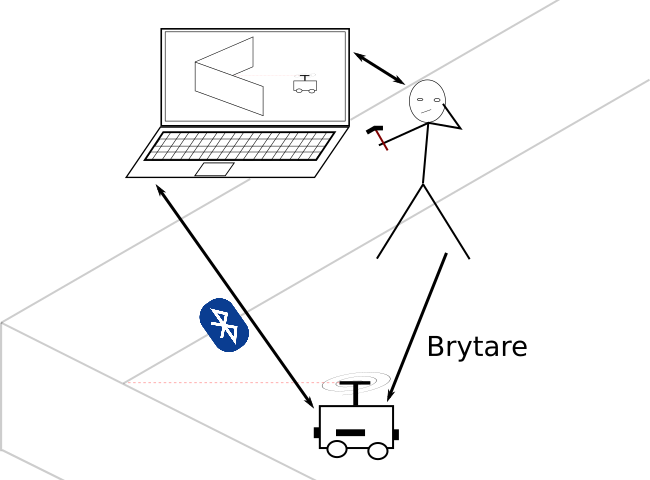
\includegraphics[width=1\textwidth]{overview.png}}
    \caption{Systemet i dess omgivning.}
    \label{fig:overview}
\end{figure}

\newpage
\section{Översikt av systemet}
Systemet är uppbyggt av tre separata moduler, samt en extern PC, enligt figur \ref{fig:modules}. Dessa delsystem kommunicerar med varandra, och med respektive moduls externa hårdvara. Ett mer detaljerat blockschema finns till varje modul, samt i sin helhet i figur \ref{fig:modulesDetailed}.
\begin{figure}[h!]
    \makebox[\textwidth][c]{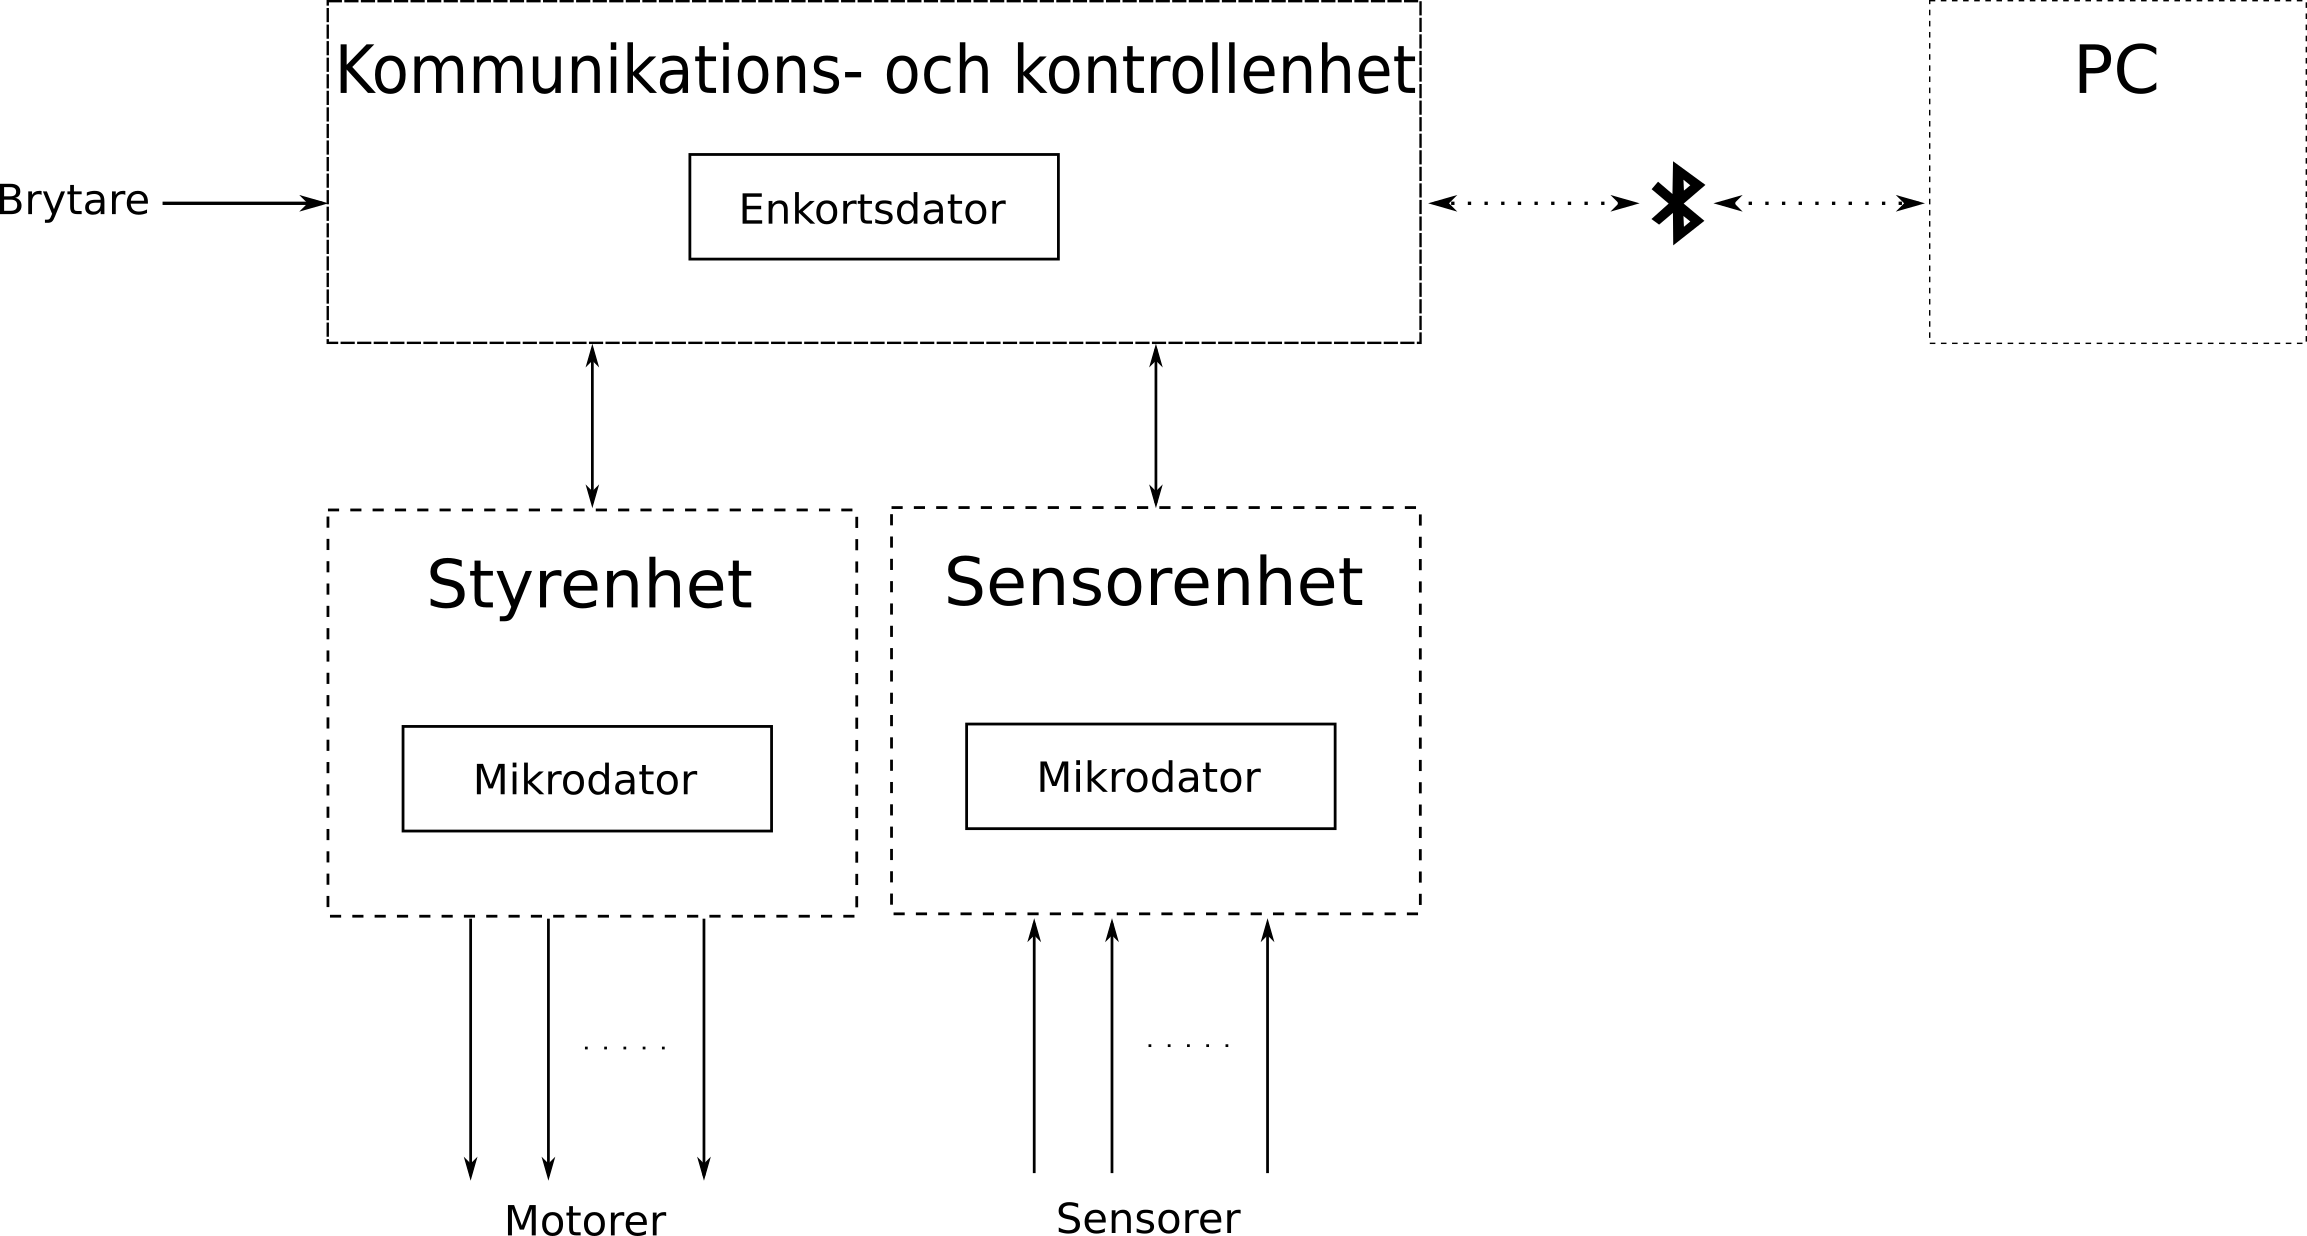
\includegraphics[width=1\textwidth]{modules.png}}
    \caption{Modulöversikt.}
    \label{fig:modules}
\end{figure}

\newpage
\section{Sensorenhet}
Sensorenheten har i uppgift att läsa in sensordata och omvandla den till ett läsligt format. Se figur \ref{fig:unitSensor} för en övergripande systemskiss för sensorenheten.
\begin{figure}[h!]
    \makebox[\textwidth][c]{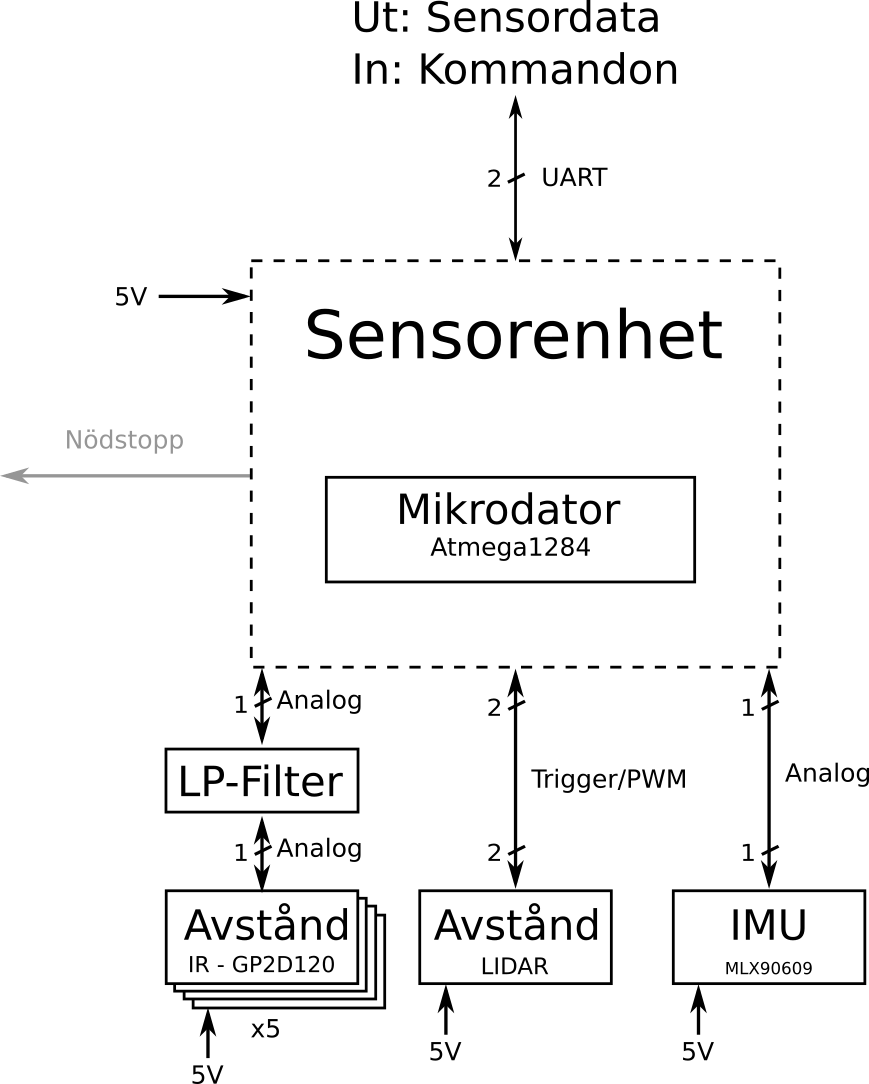
\includegraphics[width=0.6\textwidth]{sensorenhet.png}}
    \caption{Översikt över sensorenheten.}
    \label{fig:unitSensor}
\end{figure}

\noindent \begin{small}
    * Om I\textsuperscript{2}C används krävs även en logic level converter mellan 5V och 3V3 på dessa platser.\\
    ** 5V på Atmega-sidan, 3V3 krävs av sensorn.
\end{small}
\subsection{Hårdvara}

\subsubsection{Processor}
ATmega1284 används som processormodell, då den är kraftfull utan att ta det till överdrift, men även har tillräckligt med avbrottsingångar för att kunna arbeta med LIDARn och samtliga ultraljudssensorer, se \ref{sssec:sonicsensors}.

\subsubsection{Ultraljudssensor} \label{sssec:sonicsensors}
\paragraph{Alternativ 1}
En ultraljudssensor, SRF04, placeras på var och en av robotens fyra sidor och används för navigering och positionsuppskattning. Dessa behöver en utgång och en interrupt-ingång var. Se \ref{ssec:sensorInterface}. Dessa kan användas var 65:e millisekund utan risk för störningar, vilket ger oss möjlighet att läsa av $\sim15$ sensorer per sekund. Troligtvis kan de även användas med mindre eller ingen marginal mellan avläsningarna, men det kräver testning för att avgöras. En annan nackdel är att de fungerar dåligt i vinkel mot en vägg, där de antingen inte ger något värde alls, eller ett ''studsat'' värde. %http://www.robot-electronics.co.uk/htm/sonar_faq.htm

\paragraph{Alternativ 2}
Som alternativ kan IR-sensorer användas. Nackdelen är störningar i den analoga utdatan, som dessutom är ickelinjär, och fungerar på ett kortare intervall än ultraljudssensorer. Fördelen är snabbare avläsningar som troligtvis inte stör varandra. Bredden på mätstrålen är också mindre än med ultraljud.


\subsubsection{LIDAR lite v2} \label{sssec:lidar}
LIDAR är en kraftfull lasersensor som i systemet som helhet används för mätningar som kräver noggranhet. Komponenten kan kommuniceras med via en trigger-pin och PWM-output, alternativt via en I\textsuperscript{2}C-buss. I första hand kommer PWM användas.

Sensorn monteras på toppen av roboten - ovanpå ett roterande servo, som specificeras i större detalj i avsnitt \ref{ssec:servomotor}. Detta för att effektivt kunna mäta avstånd i flera vinklar.

\subsubsection{IMU} \label{sssec:imu}

\paragraph{Alternativ 1}
En enklare modul - exempelvis MLX90609 - används, via en analog ingång. Detta ger oss då endast rotationen kring z-axeln, som kan användas för att beräkna robotens riktning i rummet.

\paragraph{Alternativ 2}
En mer avancerad modul, exempelvis MPU6050, används, via en I\textsuperscript{2}C-buss. Om LIDARn implementerats med I\textsuperscript{2}C delas bussen mellan dessa två. Det ger oss i så fall både riktning och acceleration, för att mer noggrannt kunna beräkna robotens placering.% TODO: MotionMagi, handledare

\subsection{Mjukvara}

Koden ska vara skriven i C, och ska följa standarden specificerad i bilaga \ref{sec:cstandard}.

Programmet ska omvandla sensordata till ett mer läsligt format, och ska kunna skicka det vidare (se \ref{ssec:sensorInterface}).

\subsection{Gränssnitt} \label{ssec:sensorInterface}
Sensorenheten kommer behöva kommunicera med de faktiska sensorerna, samt ha ett sätt att passera vidare utdata. Sensorenheten kan ta emot uppmaningar om att starta en avläsning via samma buss som används för att rapportera mätvärden vidare.

\subsubsection{LIDAR}
LIDAR kommer i första hand använda avläsningstriggers och PWM via en gemensam pin. PWM-signalen kopplas i så fall till ett avbrott för att mäta dess längd, som används för att beräkna avståndet. Som alternativ kan också I\textsuperscript{2}C användas.

\subsubsection{I2C-buss}
Den mer avancerade av IMUerna använder I\textsuperscript{2}C. Även LIDARn kan kommunicera via I\textsuperscript{2}C. Om behov uppstår implementerar vi en I\textsuperscript{2}C-buss. Vi stödjer i så fall inte flera masters, utan behandlar processorn som den enda, med LIDAR:n och gyron som slavar.

\subsubsection{Ultraljudssensorer}
Ultraljudssensorerna (\ref{sssec:sonicsensors}) använder ett liknande gränssnitt som LIDARn, med en trigger-pin och en echo-pin som utgång. Deras utvärde beror på längden av dess höga signal, så för att garantera att vi börjar mäta omedelbart på en hög flank så ska avbrott utnyttjas. Detta uppnås genom att helt enkelt koppla denna signal till en av avbrottsportarna på processorns, för var och en av sensorerna.

\subsubsection{Utvärden/Input}
Hur tas instruktioner emot, samt hur passeras processerade mätvärden vidare?

\paragraph{Alternativ 1}
Implementera en UART-buss som endast går mellan sensorenheten och kommunikationsenheten. Se \ref{ssec:brainInterface} för mer detaljer om för och nackdelar.

\paragraph{Alternativ 2}
I\textsuperscript{2}C-bussen som eventuellt används för att kommunicera med LIDAR:n och gyron kan utnyttjas, med även processorn som slav. Enheten som tar emot data från/skickar data till sensorenheten får istället ta över rollen som master. Se \ref{ssec:brainInterface} för mer detaljer om för och nackdelar.

\newpage
\section{Styrenhet} \label{sec:system2}
Styrenheten är ansvarig för all logik och funktionalitet för robotens lågnivåstyrning. Styrenheten är länken mellan alla styrkommandon och motorerna. Se figur \ref{fig:unitMotorcontroller} för en övergripande systemskiss för styrenheten.
<<<<<<< HEAD
%TODO Ändra skissens bild så pinnar och protokoll stämmer för kommunikation med LIDAR servo
=======

%TODO Ändra protokollet mellan processor och servo från UART till PWM

>>>>>>> c5476bdd7f963dccafdd8ef9aeb6cba1e5db6dc3
\begin{figure}[h!]
    \makebox[\textwidth][c]{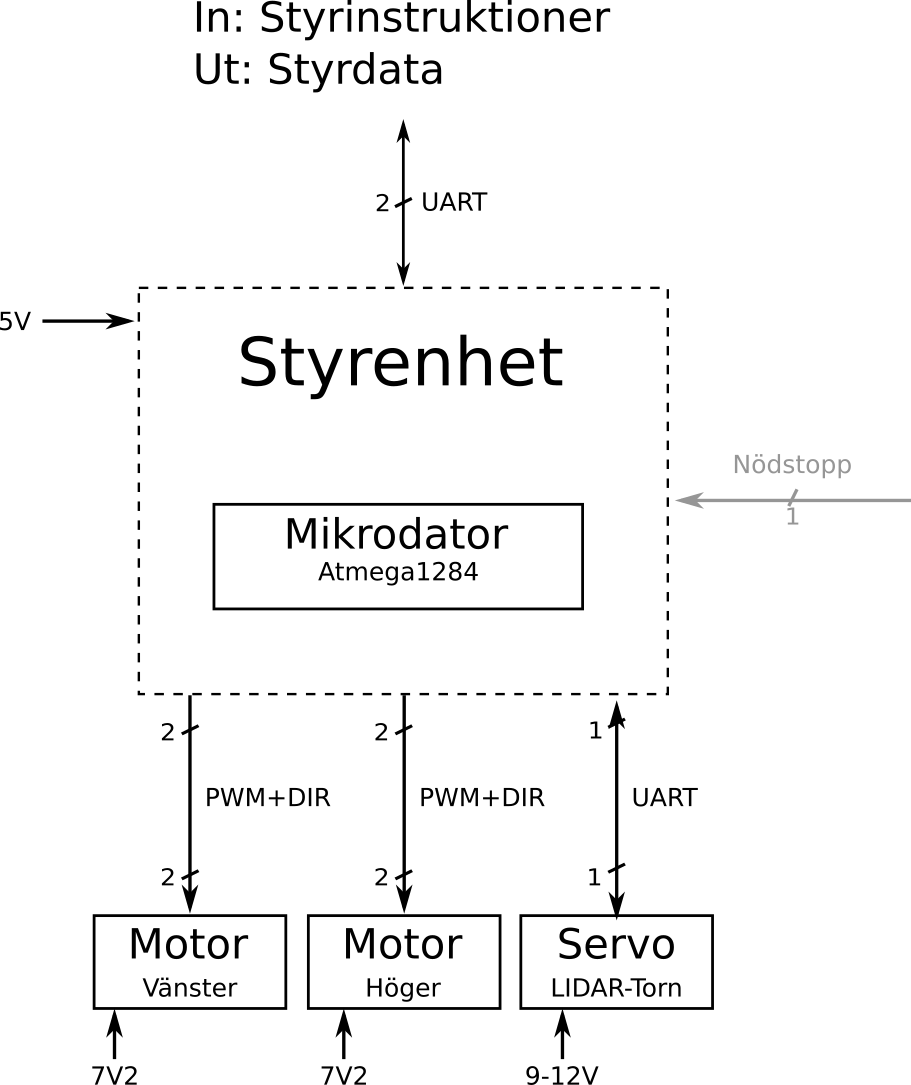
\includegraphics[width=0.6\textwidth]{styrenhet.png}}
    \caption{Översikt över styrenheten.}
    \label{fig:unitMotorcontroller}
\end{figure}
\end{small}
\subsection{Hårdvara}

\subsubsection{Processor}
<<<<<<< HEAD
Vi ska använda en Atmega1284 processor för styrmodulen. Processorn kommer totalt att kommunicera med 2 DC-motorer som sitter på chassit och 1 servo för rotation av tornet. Alla motorerna kommer kommunicera över PWM.

\subsubsection{Servo/steppermotor} \label{ssec:servomotor}
På toppen av roboten ska en sensor (se \ref{sssec:lidar}) vara monterad på en servo som tillåter sensorn att rotera. Servomotorn är en AX-12(+/A) och har två rotationslägen: ''vanlig'' och ''wheel''. Det förstnämnda tillåter oss att göra mycket exakta rotationer, men förhindrar oss från att svänga runt mer än 300 grader. Vi slipper potentiellt felaktiga värden, men kan inte titta rakt bakom oss. Då detta inte är ett stort problem används lämpligen det vanliga läget. Servot använder, enligt vissa källor, 9-12V men klarar sig enligt andra ner emot 7V. Kan alltså eventuellt kräva en step-up-krets från ~7V2 till 9-12V.

=======
Processormodellen ATmega1284.

\subsubsection{Servo/steppermotor} \label{ssec:servomotor}
På toppen av roboten ska en sensor (se \ref{sssec:lidar}) vara monterad ovanpå en roterande servo, för att tillåta sikt i flera riktningar utan att behöva rotera hela roboten. Servomotorn AX-12(+/A) används. Denna har både ett ''vanligt'' läge, och ett så kallat ''wheel''-läge som tillåter fri 360 graders rotation. Det förstnämnda tillåter oss att göra mycket exakta rotationer, men förhindrar oss från att svänga runt mer än 300 grader. Vi slipper potentiellt felaktiga värden, men kan inte titta rakt bakom oss. Då detta inte är ett stort problem används lämpligen det vanliga läget. Servot använder, enligt vissa källor, 9-12V men klarar sig enligt andra med ner emot 7V. Kan alltså eventuellt kräva en step-up-krets från ~7V2 till 9-12V.
>>>>>>> c5476bdd7f963dccafdd8ef9aeb6cba1e5db6dc3
% http://support.robotis.com/en/techsupport_eng.htm#product/dynamixel/ax_series/dxl_ax_actuator.ht

% Alternativ 3: Stepper motor med driver.

\subsubsection{Hjulmotorer}
Totalt är det fyra motorer som är monterade på chassit som går under namnet \cite{terminator}. De fyra DC-motorerna styrs parvis (höger sida och vänster sida) med hjälp av en PWM-signal samt en rotationsriktningssignal per motorpar. Sammanlagt kommer alltså 4 pinnar på Atmega1284 processorn att användas för styrning av hjulen.

\subsection{Mjukvara}

Koden ska vara skriven i C, och ska följa standarden specificerad i bilaga \ref{sec:cstandard}.

\subsection{Gränssnitt} \label{ssec:controllInterface}

\subsubsection{Styrsignaler samt styrdata}

\paragraph{Alternativ 1}
Implementera en extra UART-buss som endast går mellan styrenheten och kommunikationsenheten. Se \ref{ssec:brainInterface} för mer detaljer om för och nackdelar.

\paragraph{Alternativ 2}
I\textsuperscript{2}C-bussen som eventuellt används för att kommunicera med LIDAR:n och gyron kan utnyttjas, med även styrenheten som slav. Enheten som tar emot data från/skickar data till styrenheten får istället ta över rollen som master. Se \ref{ssec:brainInterface} för mer detaljer om för och nackdelar.

\newpage
\section{Kommunikations- och kontrollenhet} \label{sec:system3}
Kommunikations-enheten kommunicerar med de andra modulerna på roboten samt med den bärbara datorn. I denna modul ingår också kontrollenheten, som gör beräkningar relaterat till både det manuella och det autonoma läget. Se figur \ref{fig:unitBrain} för en övergripande systemskiss för kommunikations- och kontrollenheten.
\begin{figure}[h!]
    \makebox[\textwidth][c]{
\includegraphics[width=1\textwidth]{brain.png}}
    \caption{Översikt över kommunikations- och kontrollenheten.  }
    \label{fig:unitBrain}
\end{figure}
\noindent \begin{small}
* Om I\textsuperscript{2}C används krävs även en logic level converter mellan 5V och 3V3 på dessa platser.
\end{small}


\subsection{Hårdvara}

\subsubsection{Datormodell}
Då detta delsystem har hand om relativt tunga beräkningar används en Raspberry Pi 3. Vi utnyttjar Raspberryns inbyggda blåtand för trådlös kommunikation.

\subsection{Mjukvara}
Koden ska vara skriven i Python 3, och ska följa \cite{pep8}.

\subsubsection{Kommunikation}
Delsystemet är vad som i slutändan kontrollerar de olika delsystemen, och måste därför kunna skicka meddelanden mellan dessa. Den ska ha mjukvara för att kunna skicka meddelanden över de olika gränssnitten som den kopplas upp emot (se \ref{ssec:brainInterface}).

Förutom hårdvarugränssnitt ska den också kunna kommunicera med en extern PC (se \ref{sec:system4}) över blåtand, där den skickar debugdata och kartinformation, och tar emot kommandon vid manuell styrning. Mjukvara för blåtandskommunikation måste finnas.

För att hantera alla dessa meddelanden bör ett meddelandesystem implementeras. Detta görs lämpligen med en prioriterad kö, så att vissa meddelanden kan prioriteras över andra.

\subsubsection{Manuellt läge}
Roboten ska via en brytare kunna byta mellan ett autonomt och ett manuellt läge. I det manuella ska den ta emot kommandon från PC:n via blåtand (se \ref{sec:system4}) om hur den ska åka, mycket likt en radiostyrd bil. Mjukvara för att på ett korrekt sätt utföra dessa kommandon behövs.

\subsubsection{Kartritning}
Robotens huvuduppdrag i det autonoma läget är att skanna ett rum och rita en karta över det. Mjukvara för att omvandla skannerdata till ett tvådimensionellt rum, samt rutiner för att söka upp och skanna outforskade delar av rummet ska finnas.

\subsubsection{Ruttstyrning}
Roboten behöver kontinuerligt ta reda på, och leta sig till, outfoskade delar av rummet i det autonoma läget. En algoritm för att hitta ett lämpligt outforskat ställe, en för att hitta en väg dit, och en som skickar korrekta meddelanden till styrenheten (se \ref{sec:system2}) för att ta sig dit behövs.

\subsection{Gränssnitt} \label{ssec:brainInterface}

\paragraph{Alternativ 1}
Två UART-bussar används, som kopplas från kommunikations- och kontrollenhet till sensorenhet respektive styrenhet. Raspberry Pi 3 har ingen inbyggd UART som kan användas utan bland annat låsa klockfrekvensen och använda spänningsomvandlare från 5v till 3v3, och har dessutom bara en ledig om blåtand används samtidigt. Istället kan två 5 volts-kompatibla USB till UART-moduler, exempelvis CH340G eller liknande enhet, användas. Nackdelen är att UART måste implementeras på alla moduler, vilket dock verkar relativt trivialt. % TODO: LiU har förmodligen inte samma saker som kina (https://www.aliexpress.com/item/CH340-Serial-Converter-USB-To-TTL-6PIN-Module-Upgrade-Small-Plate-for-PRO-mini-Instead-of/1856263846.html). CP2102 kanske (om den är 5v-kompatibel).


\paragraph{Alternativ 2}
I\textsuperscript{2}C via samma buss som eventuella sensorer, där kommunikationsenheten agerar master. Detta gör att vi slipper implementera flera UART-bussar, men gör att både sensorer och tre moduler behöver samsas på samma buss. Har även nackdelen att kod i kommunikationsenheten behöver modifieras när sensoruppsättningen förändras, vilket minskar modulariteten.
Vid kommunikationsenheten behöver dessutom en logic level shifter användas, då Raspberry Pi använder 3v3 och övriga moduler 5v. Om I\textsuperscript{2}C inte används för LIDAR eller IMU har en onödigt komplicerad buss utvecklats i onödan.

\newpage
\section{ Mjukvara på PC} \label{sec:system4}
Detta delsystem kommunicerar med Kommunikations- och kontrollenheten (se \ref{sec:system3}) för att ta emot diagnostisk data, den upptäckta kartan, samt ge instruktioner vid manuellt läge. Se figur \ref{fig:unitPC} för en övergripande systemskiss för PC-mjukvaran.

\begin{figure}[h!]
    \makebox[\textwidth][c]{
\includegraphics[width=0.4\textwidth]{PC.png}}
    \caption{Översikt över PCn.}
    \label{fig:unitPC}
\end{figure}
\subsection{Hårdvara}
En godtycklig PC med Python-3-support, skärm, tangentbord, och blåtandsmodul.

\subsection{Mjukvara}

Koden ska vara skriven i Python 3, och ska följa \cite{pep8}.

Då grafiska element (snarare än kommandoraden) måste utnyttjas så införskaffas ett lämpligt grafikbibliotek.

\subsubsection{Input}
PC-mjukvaran tar emot sensordata, styrdata och kartdata från kommunikationsenheten via blåtand. Den tar också emot instruktioner från mus och tangentbord. 

\subsubsection{Output}
Mjukvaran skickar styrkommandon samt uppmaning om att läsa av sensorerna till roboten i dess manuella läge. Den kan också skicka kommandon om att växla mellan autonomt och manuellt läge, som då går före den fysiska brytaren på roboten.

Informationen som tas emot från roboten presenteras i ett grafiskt gränssnitt.

\subsection{Gränssnitt} \label{ssec:PCInterface}

PC:n utnyttjar, som omnämnt, en blåtandsmodul.

\newpage
\begin{appendices}

\section{Detaljerat blockschema}
% TODO: Riktig titel
\begin{figure}[h!]
    \makebox[\textwidth][c]{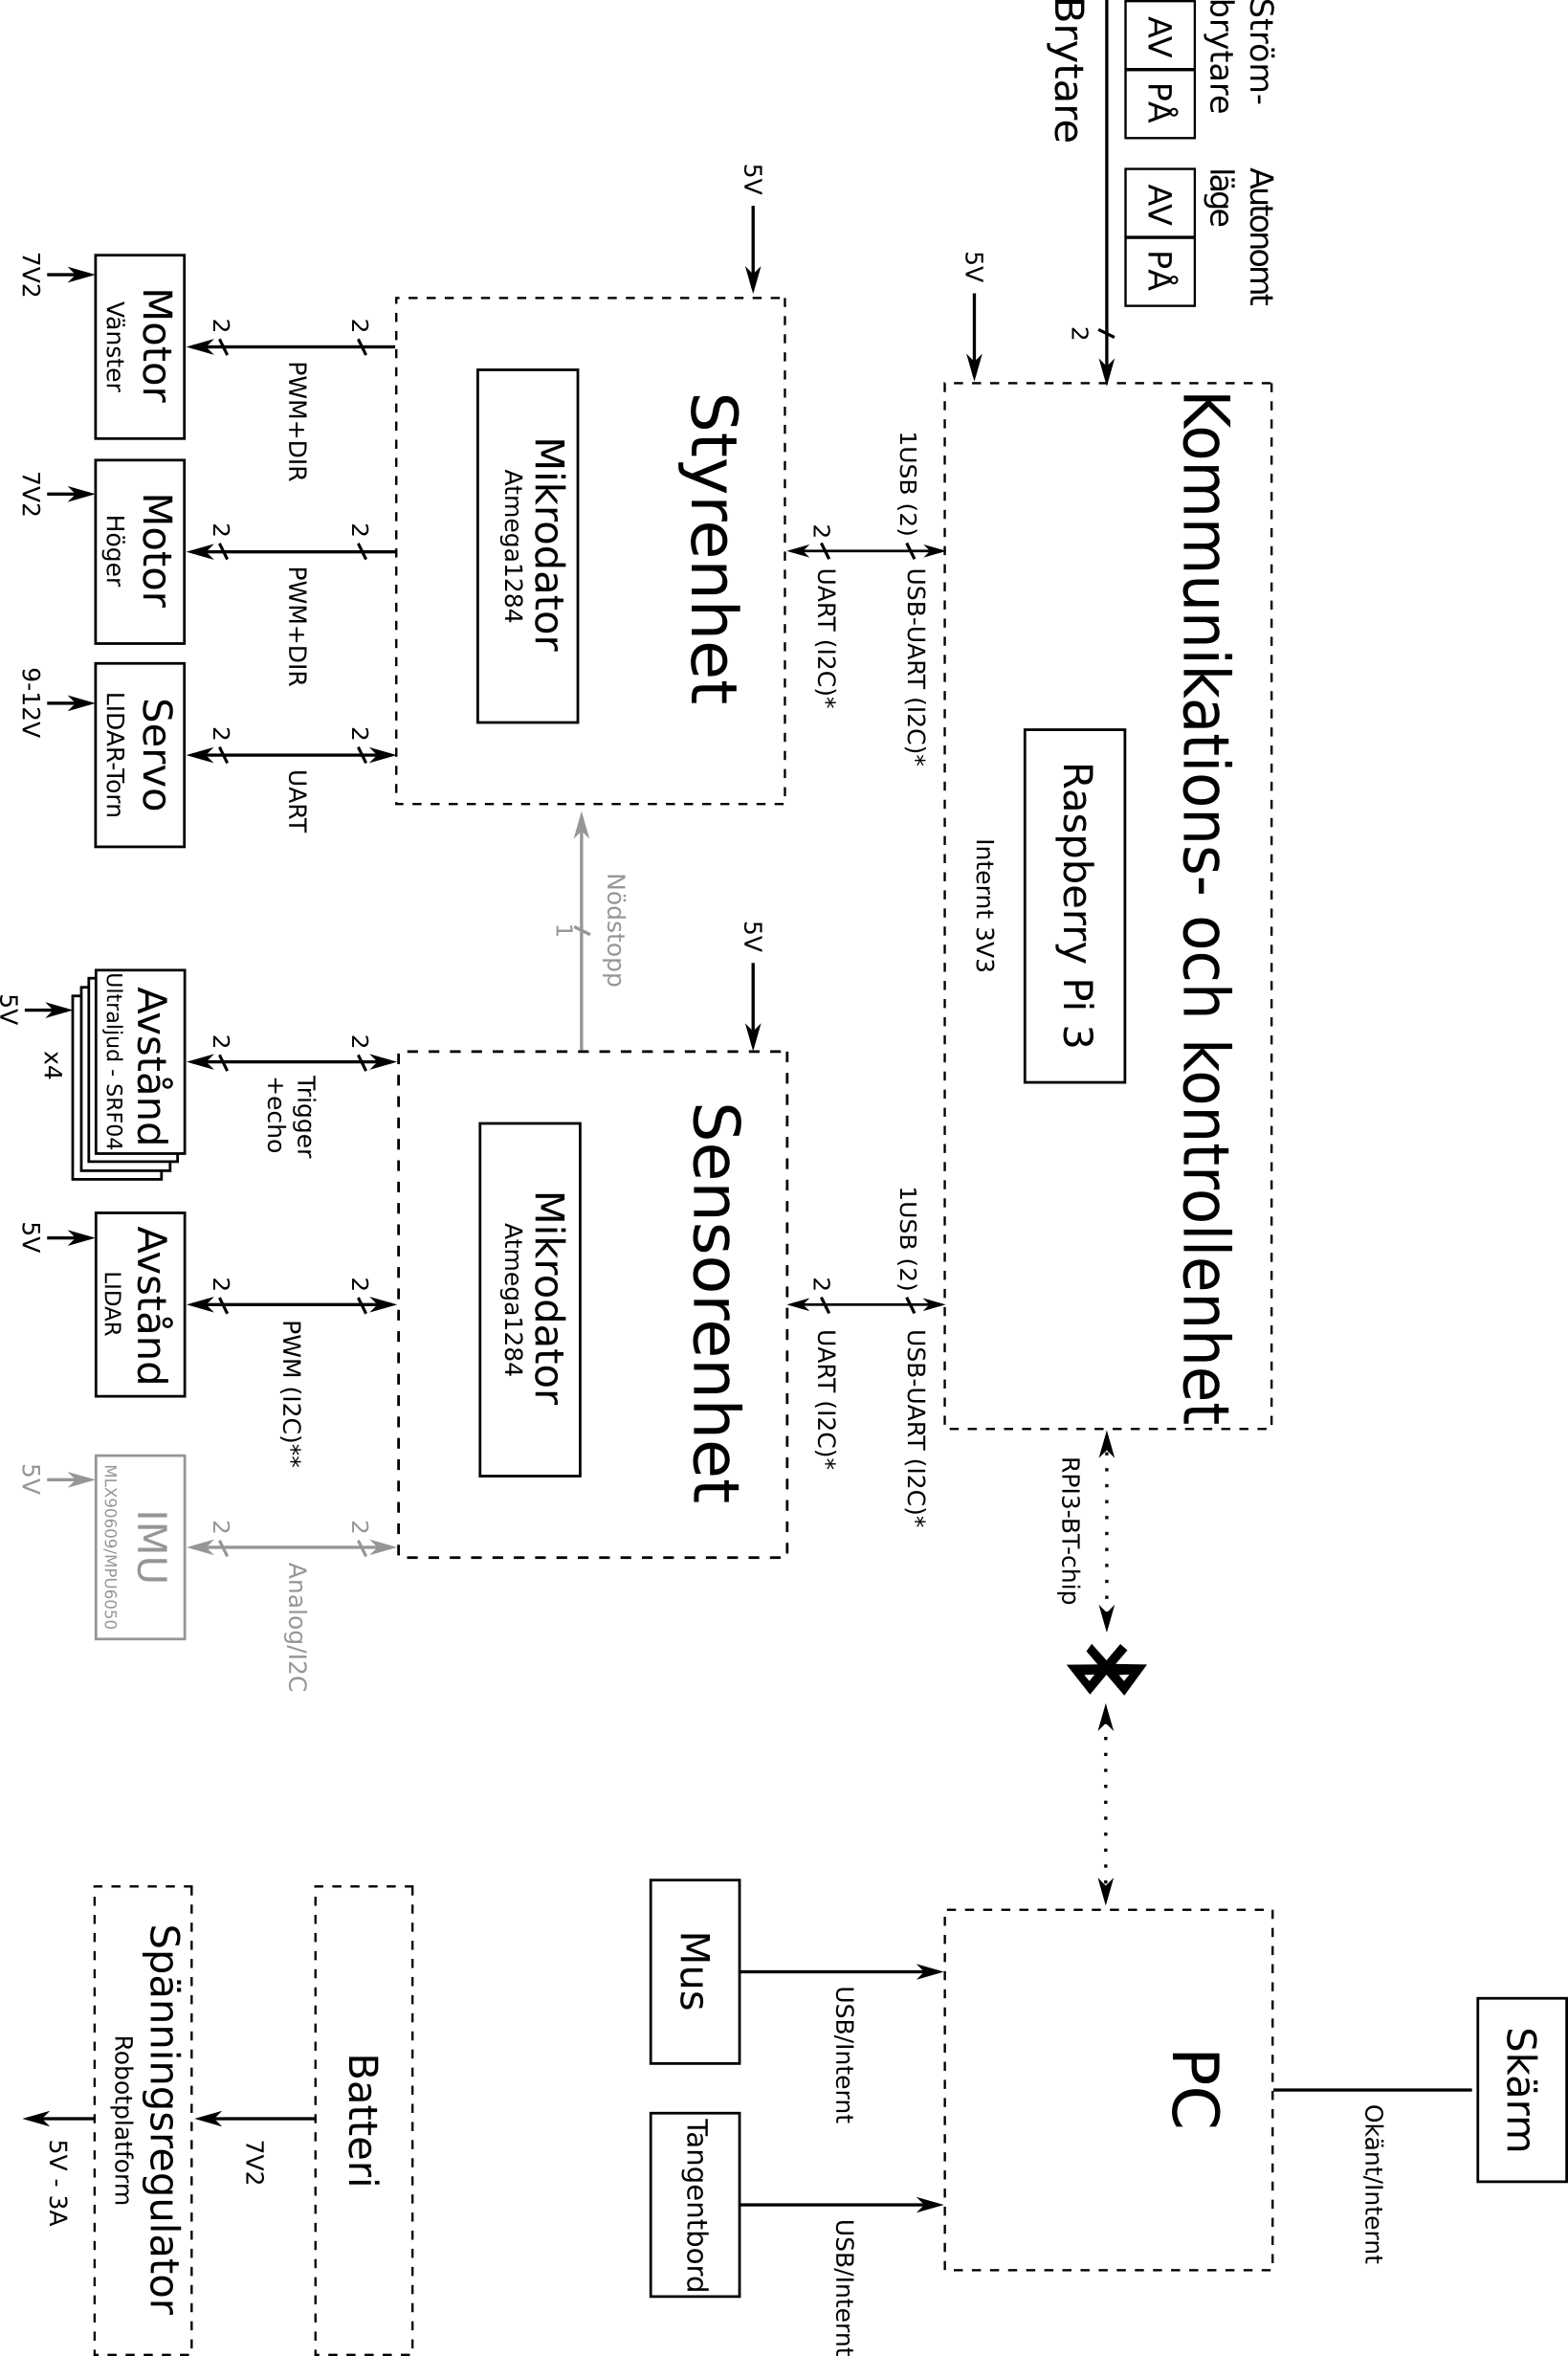
\includegraphics[width=0.85\textwidth]{modules_detail.png}}
    \caption{Detaljerat blockschema över systemet.}
    \label{fig:modulesDetailed}
\end{figure}

\noindent \begin{small}
    * Om I\textsuperscript{2}C används krävs även en logic level converter mellan 5V och 3V3 på dessa platser.\\
    ** 5V på Atmega-sidan, 3V3 krävs av sensorn.
\end{small}

\section{C-standard} \label{sec:cstandard}
Som kodstandard för C används \cite{cstandard} med några smärre tillägg och ändringar:

\begin{itemize}
    \item Indenteringar sker med exakt fyra stycken mellanslag.
    \item Namn på funktioner, typedef, variabler, strukter, unioner, och enums ska vara i lower camel case.
    \item Namn på \#define's, enum-konstanter, och macrofunktioner ska vara i all-caps med ord separerade av underscore.
    \item Typedef:ade namn ska avslutas med "\_t".
    \item Globala namn ska \textit{ej} påbörjas med ett prefix som identiferar vilken modul de tillhör.
    \item Dokumentationskommentarer för funktioner och dylikt ska inledas med "/*" följt av tom rad, med textrader inledda med "{ }* ". Hela kommentaren avslutas med en rad som endast innehåller "{ }*/".
\end{itemize}

\end{appendices}

\clearpage
\addcontentsline{toc}{section}{Referenser} %append references section at this location to TOC
\printbibliography
\end{document}
